
\title{Taler: \\ Usable, privacy-preserving payments for the Web}
 \author{
 Jeffrey Burdges \\ \and
 Florian Dold \\ \and
 Christian Grothoff \\ \and
 Marcello Stanisci
}
\date{\today}

\documentclass[twoside,letterpaper]{sigalternate}
\usepackage[margin=1in]{geometry}
\usepackage[utf8]{inputenc}
\usepackage{url}
\usepackage{tikz}
\usepackage{eurosym}
\usepackage{listings}
\usepackage{graphicx}
\usepackage{wrapfig}
%\usepackage{caption}
\usepackage{subcaption}
\usepackage{url}

\usetikzlibrary{shapes,arrows}
\usetikzlibrary{positioning}
\usetikzlibrary{calc}

\begin{document}
\maketitle

\section{System overview}

Transactions on the Internet, such as sending an e-mail or reading a
Web site, tend to be of smaller value than traditional transactions
involving the exchange of physical goods. Thus we are faced with the
challenge of reducing the mental and technical overheads of existing
payment systems to handle micro-payments.  Addressing this problem is
urgent: ad-blocking technology is eroding advertising as a substitute
for micro-payments, and the Big Data business model where citizens pay
with their private information in combination with the deep state
hastens our society's regression towards
post-democracy~\cite{rms2013democracy}.

Taler is a new electronic online payment system which provides
anonymity for customers.  Here, {\em anonymous} simply means that the
payment system does not require any personal information from the
customer, and that different transactions by the same customer are
unlinkable.  For strong anonymity, Taler usually needs to be used in
combination with existing techniques (such as~\cite{apod}) to avoid
circumstances leaking information about the customer's identity.  The
fact that the user does not need to authenticate and that the merchant
thus never learns sensitive personal information about the customer
improves usability: the payment process is simplified and the
merchant's security requirements are dramatically reduced.

Taler uses blind signatures~\cite{chaum1983blind} to create digital
coins, and a new ``refresh'' protocol to allow giving change and
refunds while maintaining unlinkability.  We will not go into the
details of Taler's cryptographic protocols here\footnote{Full
documentation at \url{https://api.taler.net/}} and instead focus on
the interaction sequences to explain how the system works from the
perspective of customers and merchants in the Taler
system (Figure~\ref{fig:system}).

\begin{figure}[t!]
\centering
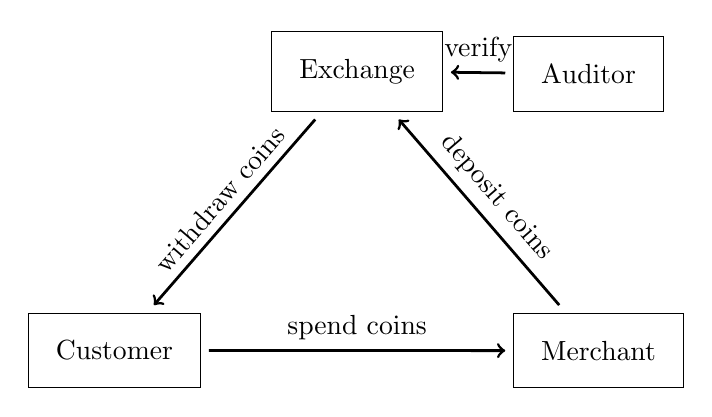
\begin{tikzpicture}
 \tikzstyle{def} = [node distance=3em and 5em, inner sep=1em, outer sep=.3em];
 \node (origin) at (0,0) {};
 \node (exchange) [def,above=of origin,draw]{Exchange};
 \node (customer) [def, draw, below left=of origin] {Customer};
 \node (merchant) [def, draw, below right=of origin] {Merchant};
 \node (auditor) [def, draw, above right=of origin]{Auditor};

 \tikzstyle{C} = [color=black, line width=1pt]

 \draw [<-, C] (customer) -- (exchange) node [midway, above, sloped] (TextNode) {withdraw coins};
 \draw [<-, C] (exchange) -- (merchant) node [midway, above, sloped] (TextNode) {deposit coins};
 \draw [<-, C] (merchant) -- (customer) node [midway, above, sloped] (TextNode) {spend coins};
 \draw [<-, C] (exchange) -- (auditor) node [midway, above, sloped] (TextNode) {verify};

\end{tikzpicture}
\caption{Taler system overview.}
\label{fig:system}
\end{figure}

\newpage
\section{Customer perspective}

In Taler, customers use a {\em wallet} to withdraw (Figure
~\ref{fig:taler-withdraw}), hold, and spend (Figure~\ref{fig:taler-pay})
coins.  Withdrawing coins requires the customer to authenticate
and to optionally authorize the specific transaction.
Afterwards, the customer can anonymously spend his coins by
visiting merchants without having to authenticate for each
transaction (Figure~\ref{fig:taler-pay}).

\begin{figure}[h!]
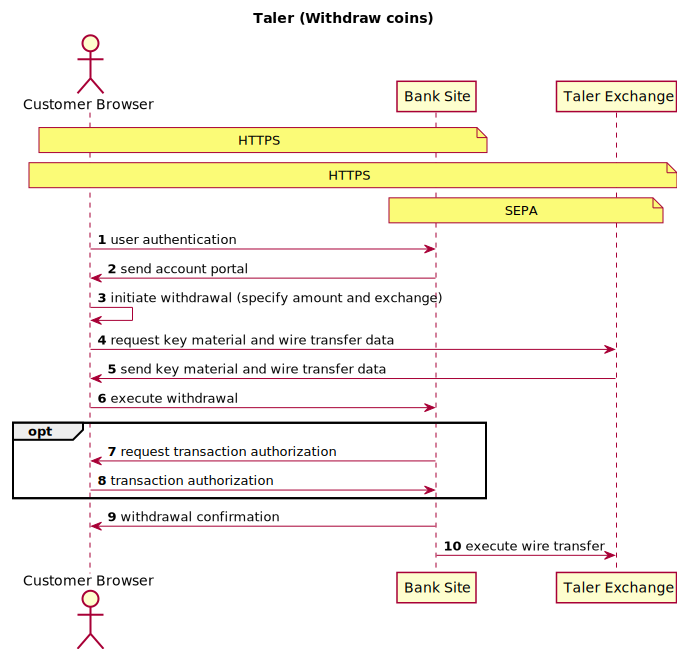
\includegraphics[width=0.45\textwidth]{figs/taler-withdraw.pdf}
\caption{Withdrawing coins with Taler.}
\label{fig:taler-withdraw}
\end{figure}


\begin{figure*}[t!]
\begin{center}
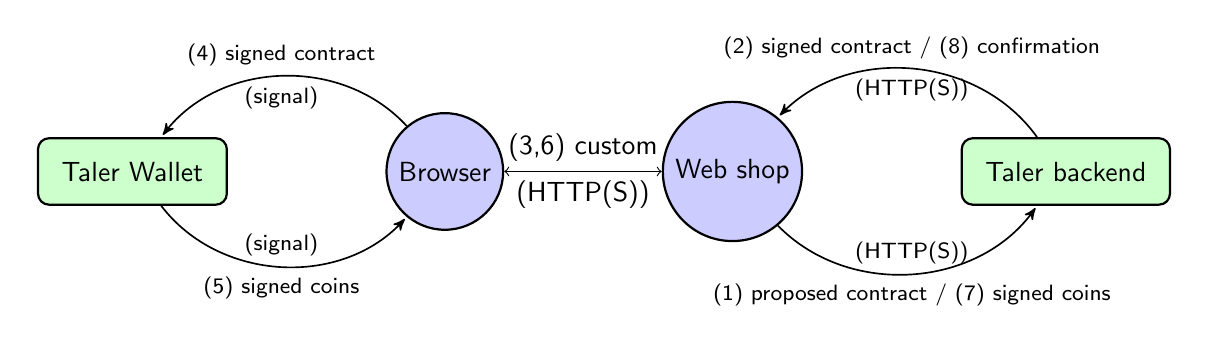
\begin{tikzpicture}[
  font=\sffamily,
  every matrix/.style={ampersand replacement=\&,column sep=2cm,row sep=2cm},
  source/.style={draw,thick,rounded corners,fill=green!20,inner sep=.3cm},
  process/.style={draw,thick,circle,fill=blue!20},
  sink/.style={source,fill=green!20},
  datastore/.style={draw,very thick,shape=datastore,inner sep=.3cm},
  dots/.style={gray,scale=2},
  to/.style={->,>=stealth',shorten >=1pt,semithick,font=\sffamily\footnotesize},
  every node/.style={align=center}]

  % Position the nodes using a matrix layout
  \matrix{
    \node[source] (wallet) {Taler Wallet};
      \& \node[process] (browser) {Browser};
      \& \node[process] (shop) {Web shop};
      \& \node[sink] (backend) {Taler backend}; \\
  };

  % Draw the arrows between the nodes and label them.
  \draw[to] (browser) to[bend right=50] node[midway,above] {(4) signed contract}
      node[midway,below] {(signal)} (wallet);
  \draw[to] (wallet) to[bend right=50] node[midway,above] {(signal)}
      node[midway,below] {(5) signed coins} (browser);
  \draw[<->] (browser) -- node[midway,above] {(3,6) custom}
      node[midway,below] {(HTTP(S))} (shop);
  \draw[to] (shop) to[bend right=50] node[midway,above] {(HTTP(S))}
      node[midway,below] {(1) proposed contract / (7) signed coins} (backend);
  \draw[to] (backend) to[bend right=50] node[midway,above] {(2) signed contract / (8) confirmation}
      node[midway,below] {(HTTP(S))} (shop);
\end{tikzpicture}
\end{center}
 \caption{Both the customer's client and the merchant's server execute
          sensitive cryptographic operations in a secured
          background/backend that is protected against direct access.
          Interactions between the Taler components
          (Figure~\ref{fig:system}) are not shown.  Existing system
          security mechanisms are used to isolate the cryptographic
          components (boxes) from the complex rendering logic
          of existing Web applications (circles).}
 \label{fig:frobearch}
\end{figure*}


\begin{figure}[b!]
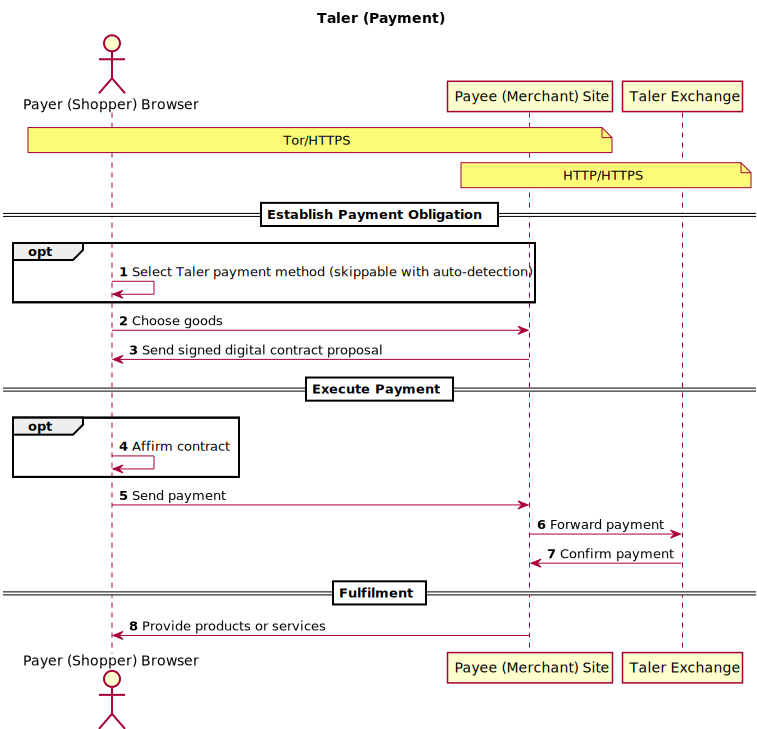
\includegraphics[width=0.45\textwidth]{figs/taler-pay.pdf}
\caption{Payment processing with Taler.}
\label{fig:taler-pay}
\end{figure}

\newpage
\section{Merchant perspective}

A new payment system must also be easy to deploy for merchants.
Figure~\ref{fig:frobearch} shows how the secure payment components of
Taler interact with the logic of existing Web shops.  First, the Web shop
front-end is responsible for constructing the shopping cart.  For this,
the shop front-end generates the usual Web pages which are shown to the
user's browser client front-end.  Once the order has been constructed,
the shop front-end gives a {\em proposed contract} in JSON format to
the payment backend, which signs it and returns it to the front-end.
The front-end then transfers the signed contract over the network, and
passes it to the wallet.  Here, the wallet operates from a secure {\em
background} on the client side, which allows the user to securely
accept the payment, and to perform the cryptographic operations in a
context that is protected from the Web shop.  If the user accepts, the
resulting signed coins are transferred from the client to the server,
again by a protocol that the merchant can customize to fit the
existing infrastructure.

Instead of adding any cryptographic logic to the merchant front-end,
the generic Taler merchant backend allows the implementor to delegate
handling of the coins to the payment backend, which validates the
coins, deposits them at the exchange, and finally validates and
persists the receipt from the exchange.  The merchant backend then
communicates the result of the transaction to the front\-end, which is
then responsible for executing the business logic to fulfill the
order.  As a result of this setup, the cryptographic details of the
Taler protocol do not have to be re-implemented by each merchant.
Instead, existing Web shops implemented in a multitude of programming
languages can rather trivially add support for Taler by {\bf (1)} upon
request, generating a contract in JSON based on the shopping cart,
{\bf (2)} allowing the backend to sign the contract before sending it
to the client, {\bf (7)} passing coins received in payment for a
contract to the backend and {\bf (8)} executing fulfillment business
logic if the backend confirms the validity of the payment.

To setup a Taler backend, the merchant only needs to let it know the
respective wire transfer routing details, such as an IBAN number.  The
customer's authentication of the Web shop continues to rely upon
\mbox{HTTPS}/X.509.

\section{Conclusion}

We encourage everyone to try our prototype for Taler
at \url{https://demo.taler.net/}.

% These APIs are all RESTful in the modern sense because that greatly
% simplify integrating Taler with web shops and browsers.

\section*{Acknowledgements}

This work benefits from the financial support of the Brittany Region
(ARED 9178) and a grant from the Renewable Freedom Foundation.


%\newpage

\bibliographystyle{abbrv}
\bibliography{ui,btc,taler,rfc}

\end{document}
